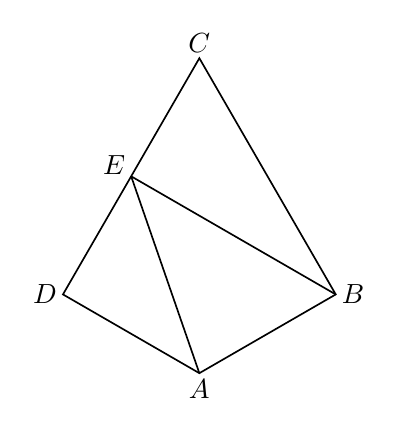
\begin{tikzpicture}[x=1cm,y=1cm,font=\normalsize,
 geometry edge/.style={solid,line width=.6pt},
 geometry mark/.style={solid,line width=.6pt},
 geometry label/.style={font=\normalsize,inner sep=2pt}]
\coordinate (A) at (0,0);
\coordinate (B) at (1.7320508075688774,1);
\coordinate (C) at (0,4);
\coordinate (D) at (-1.7320508075688772,1);
\coordinate (E) at (-0.8660254037844384,2.5);
\draw[geometry edge] (C)--(B)--(A)--(D)--cycle;
\draw[geometry edge] (E)--(B);
\draw[geometry edge] (E)--(A);
\node[geometry label,above] at (C) {$C$};
\node[geometry label,right] at (B) {$B$};
\node[geometry label,below] at (A) {$A$};
\node[geometry label,left] at (D) {$D$};
\node[geometry label,left,yshift=4pt] at (E) {$E$};
\end{tikzpicture}
